%\section{3D motion and its 2D projection}
\chapter{3D Motion and Its 2D Projection}
\label{chapter:3D_motion_and_its_2D_projection}
%Derive the projection of 2D flow from 3D flow. 



\section{Introduction}

As objects move in the world, or as the camera moves, the projection of the dynamic scene into the two-dimensional (2D) camera plane produces a sequence of temporally varying pixel brightness. Before diving into how to estimate motion from pixels, it is useful to understand the image formation process. Studying how three-dimensional (3D) motion projects into the camera will allow us to understand what the difference is between a moving camera or a moving object and what types of constraints one might be able to use to estimate motion.


\section{3D Motion and Its 2D Projection}

A 3D point will follow a trajectory $\mathbf{P}(t) = (X(t),Y(t),Z(t))$, in  camera coordinates (\fig{\ref{fig:optical_flow_basic_motion_point}}). As the point moves, it has an instantaneous 3D velocity of $\dot{\mathbf{P}} = (\dot{X}(t), \dot{Y}(t), \dot{Z}(t))$. The projection of this point into the image plane location is $\mathbf{p}(t) = (x(t),y(t))$ and its projection will move with the 2D instantaneous velocity $\dot{\mathbf{p}} = (\dot{x}(t), \dot{y}(t))$, where all the derivatives are done with respect to time, $t$.

\vspace{-.2in}
\begin{figure}[h!]
    \centerline{
        \includegraphics[width=.5\linewidth]{figures/optical_flow/basic_motion_point.eps}
    }
    \caption{A 3D point, $\mathbf{P}$, moving in the world projects a 2D moving point, $\mathbf{p}$, into the camera plane.}
    \label{fig:optical_flow_basic_motion_point}
\end{figure}
\vspace{-.2in}

Using the equations of perspective projection $x=f X/Z$ and $y=f Y/Z$ (assuming that the camera is at the origin of the world-coordinate system), we can derive the equations of how the instantaneous velocity in the camera plane relates to the point motion in 3D world coordinates:
\begin{eqnarray}
    \dot{x} & = & f \frac{\dot{X} Z - \dot{Z} X}{Z^2} = \frac{f \dot{X} - \dot{Z} x}{Z}\\
    \dot{y} & = & f \frac{\dot{Y} Z - \dot{Z} Y}{Z^2} = \frac{f \dot{Y} - \dot{Z} y}{Z}
\end{eqnarray}
The second expression is obtained by using $x=f \, X/Z$ and $y=f \, Y/Z$, which removes the dependency on the world coordinates $X$ and $Y$. Note that $f$ is the focal length. In many derivations, the notation is simplified by setting the focal length $f=1$. Here we will keep it to make explicit which factors depend on the camera parameters and which ones do not.
%\begin{equation}
%\dot{x} = f \frac{\dot{X} Z - \dot{Z} X}{Z^2} = \frac{f \dot{X} - \dot{Z} x}{Z}
%\end{equation}
We can write the last two equations in matrix form as:
\begin{align}
    \begin{bmatrix}
        \dot{x} \\
        \dot{y}
    \end{bmatrix}
    = \frac{1}{Z}
    \begin{bmatrix}
        f & 0 & -x \\
        0 & f & -y
    \end{bmatrix}
    \begin{bmatrix}
        \dot{X} \\
        \dot{Y} \\
        \dot{Z}
    \end{bmatrix}
    \label{eq:motionprojection}
\end{align}
This expression reveals a number of interesting properties of the optical flow and how it relates to motion in the world. For instance, points that move parallel to the camera plane ($\dot{Z} = 0$) will project to a motion parallel to the motion in 3D but with a magnitude that will be inversely proportional to the distance $Z$:
\begin{align}
    \begin{bmatrix}
        \dot{x} \\
        \dot{y}
    \end{bmatrix}
    = \frac{f}{Z}
    \begin{bmatrix}
        \dot{X} \\
        \dot{Y}
    \end{bmatrix}
    \label{eq:parallelmotion}
\end{align}

%\begin{figure}
%\centerline{
%\includegraphics[width=1\linewidth]{figures/optical_flow/motion_projection.eps}
%} 
%\caption{a) scene with three vehicles moving with the same speed, $V$, parallel to the camera plane. The blue and black cars move inside the plane $Z=d$, and the red car moves in the plane $Z=2d$. b) After projection in the camera plane, the objects close to the camera move with a speed of $v=f V/d$. The red car, which is twice as far from the camera, will have half the image size and it will move with speed $v/2$. The size of the cars will not change as they move.} 
%\label{fig:parallel_objects}
%\end{figure}

For points moving parallel to the $Z$ axis ($\dot{X} = \dot{Y} = 0$) we get:
\begin{align}
    \begin{bmatrix}
        \dot{x} \\
        \dot{y}
    \end{bmatrix}
    = -\frac{\dot{Z}}{Z}
    \begin{bmatrix}
        x \\
        y
    \end{bmatrix}
    \label{eq:forward_objects}
\end{align}
Points at the same distance $Z$ from the camera, moving away or towards the camera ($\dot{Z} \neq 0$, and $\dot{X} = \dot{Y} = 0$), with the same velocity will project into points moving at different velocities on the image plane.


\Fig{\ref{fig:examples_3d_moving_points}} illustrates the geometry of the projection of 3D motion into the camera for points moving parallel to the camera plane (\fig{\ref{fig:examples_3d_moving_points}}[left]) and parallel to the optical axis of the camera (\fig{\ref{fig:examples_3d_moving_points}}[right]). The arrows at the image plane show the imaged scene velocities.
%\vspace{-.1in}
\begin{figure}
    \centerline{
        \includegraphics[width=1\linewidth]{figures/optical_flow/examples_3d_moving_points.eps}
    }
    \caption{(left) Geometry of the projection of 3D motion into the camera for points moving parallel to the camera plane, and (right) parallel to the optical axis of the camera.}
    \label{fig:examples_3d_moving_points}
\end{figure}
%\vspace{-.1in}

%\section{Camera motion}

Let's examine a few scenarios in a bit more detail to gain some familiarity with the relationship between 3D motion and the projected 2D motion field.

\subsection{Vanishing Point}

Let's consider a point moving in a straight line in 3D with constant velocity over time: $\dot{\mathbf{P}} = (V_X, V_Y, V_Z)^\transpose$. At each time instant, $t$, the point location will be $\mathbf{P}(t) = (X+V_Xt, Y+V_Yt, Z+V_Zt)^\transpose$, and its 2D projection:
\begin{eqnarray}
    x(t) & = & f \frac{X + V_X t}{Z + V_Z t}\\
    y(t) & = & f \frac{Y + V_Y t}{Z + V_Z t}
\end{eqnarray}
If $\dot{Z}=0$, then the projected point will move with constant velocity over time, as shown in \eqn{\ref{eq:parallelmotion}}. If $\dot{Z} \neq  0$, then, as time goes to infinity, the point will converge to a {\bf vanishing point}:
\index{Vanishing point}
\begin{eqnarray}
    \lim_{t \to \infty} x(t)  & = & f \frac{V_X}{V_Z} = x_{\infty}\\
    \lim_{t \to \infty} y(t) & = & f \frac{V_Y}{V_Z} = y_{\infty}
    \label{eq:motionvanishingpoint}
\end{eqnarray}

%\begin{equation}
%\lim_{t \to \infty} \left( x(t),y(t) \right) = \left( f \frac{V_X}{V_Z}, f \frac{V_Y}{V_Z} \right) = (x_{\infty}, y_{\infty}) = \mathbf{p}_{\infty}
%\label{eq:motionvanishingpoint}
%\end{equation}

The following sketch (\fig{\ref{fig:flying_bird}}) shows Gibson's bird (see \fig{\ref{fig:gibson_bird}}) flying away from the camera along a straight line. In the camera the bird gets smaller as it flies away until it disappears at the vanishing point. In this drawing the vanishing point is within the view of the camera.
%\vspace{-.2in}

\begin{figure}[h!]
    \centerline{
        \includegraphics[width=1\linewidth]{figures/optical_flow/flying_bird.eps}
    }
    \caption{Projection onto the camera plane of the sequence produced by a bird flying away. The bird will vanish at the {\bf vanishing point}.}
    \label{fig:flying_bird}
\end{figure}
%\vspace{-.2in}

The vanishing point is the location $\mathbf{p}_{\infty}=(x_{\infty}, y_{\infty})^\transpose$ where the moving point slowly converges to. The location of the vanishing point is independent of the point location at time $t=0$, and it only depends on the 3D velocity vector, $\mathbf{V}$. Therefore, if the scene contains multiple points at different locations moving with the same velocity, they will converge to the same vanishing point.

\subsection{Camera Translation}

Let's now assume that the scene is static and that only the camera is moving. In this case, all the observed motion in the image will be due to the motion of the camera.

Let's assume the camera is moving in a straight line with a velocity $\dot{\mathbf{T}} = \mathbf{V} = (V_X,V_Y,V_Z)^\transpose$. The translation of the camera after time $t$ will be $\mathbf{T} = \mathbf{V} t$. A point in space $\mathbf{P} = (X,Y,Z)^\transpose$, will move with velocity, relative to the camera, equal to $\dot{\mathbf{P}} = -\mathbf{V}$.  The moving camera is equivalent to the case where all the scene points move relative to the camera with the same velocity.

The 2D motion field by using \eqn{\ref{eq:motionprojection}} is:
\begin{align}
    \begin{bmatrix}
        \dot{x} \\
        \dot{y}
    \end{bmatrix}
    = \frac{1}{Z}
    \begin{bmatrix}
        -f & 0  & x \\
        0  & -f & y
    \end{bmatrix}
    \begin{bmatrix}
        V_X \\
        V_Y \\
        V_Z
    \end{bmatrix}
    \label{eq:2d_motion_field_equation}
\end{align}

We can also express the same relationship by making the contribution of the camera coordinates more explicit. We can do this by rearranging the terms in \eqn{\ref{eq:2d_motion_field_equation}}, resulting in:
\begin{align}
    \begin{bmatrix}
        \dot{x} \\
        \dot{y}
    \end{bmatrix}
    = -\frac{f}{Z}
    \begin{bmatrix}
        V_X \\
        V_Y
    \end{bmatrix}
    +
    \frac{V_Z}{Z}
    \begin{bmatrix}
        x \\
        y
    \end{bmatrix}
\end{align}

\Eqn{\ref{eq:2d_motion_field_equation}} gives a generic expression for the observed motion in the camera plane produced by a moving camera undergoing a translation (we will see later what happens if we also have camera rotation). But let's first look at a few specific scenarios with a camera following simple translation trajectories (and no rotations).

\subsubsection{Lateral camera motion}
%~\\
Consider a camera translating laterally, as shown in \fig{\ref{fig:camera_lateral_translation}}. This will happen if you are looking through a side window of a car at the scene passing by. In this case, the forward velocity is zero, $V_Z=0$.

\begin{figure}
    \centerline{
        \includegraphics[width=1\linewidth]{figures/optical_flow/camera_lateral_translation.eps}
    }
    \caption{Lateral camera motion parallel to the camera plane.}
    \label{fig:camera_lateral_translation}
\end{figure}

Under lateral camera motion, using \eqn{\ref{eq:parallelmotion}}, we have the following relationship between the velocity of a 3D point and the apparent velocity of its projection in the image plane:
%\begin{eqnarray}
%\dot{x} & = &  -f\frac{V_X}{Z} \\
%\dot{y} & = &  -f\frac{V_Y}{Z}
%\label{eq:motionprojection}
%\end{eqnarray}

\begin{align}
    \begin{bmatrix}
        \dot{x} \\
        \dot{y}
    \end{bmatrix}
    =
    -\frac{f}{Z}
    \begin{bmatrix}
        V_X \\
        V_Y
    \end{bmatrix}
\end{align}

The motion field depends on the depth at each location $Z$ as illustrated in \fig{\ref{fig:camera_lateral_translation_flow}}. Objects close to the camera will appear moving faster than objects farther away. Objects that are very far will appear as not moving. This parallax effect is the same one used in stereo vision to recover depth. The 2D motion in the image place is in the opposite direction to the camera motion.

\begin{figure}[h!]
    \centerline{
        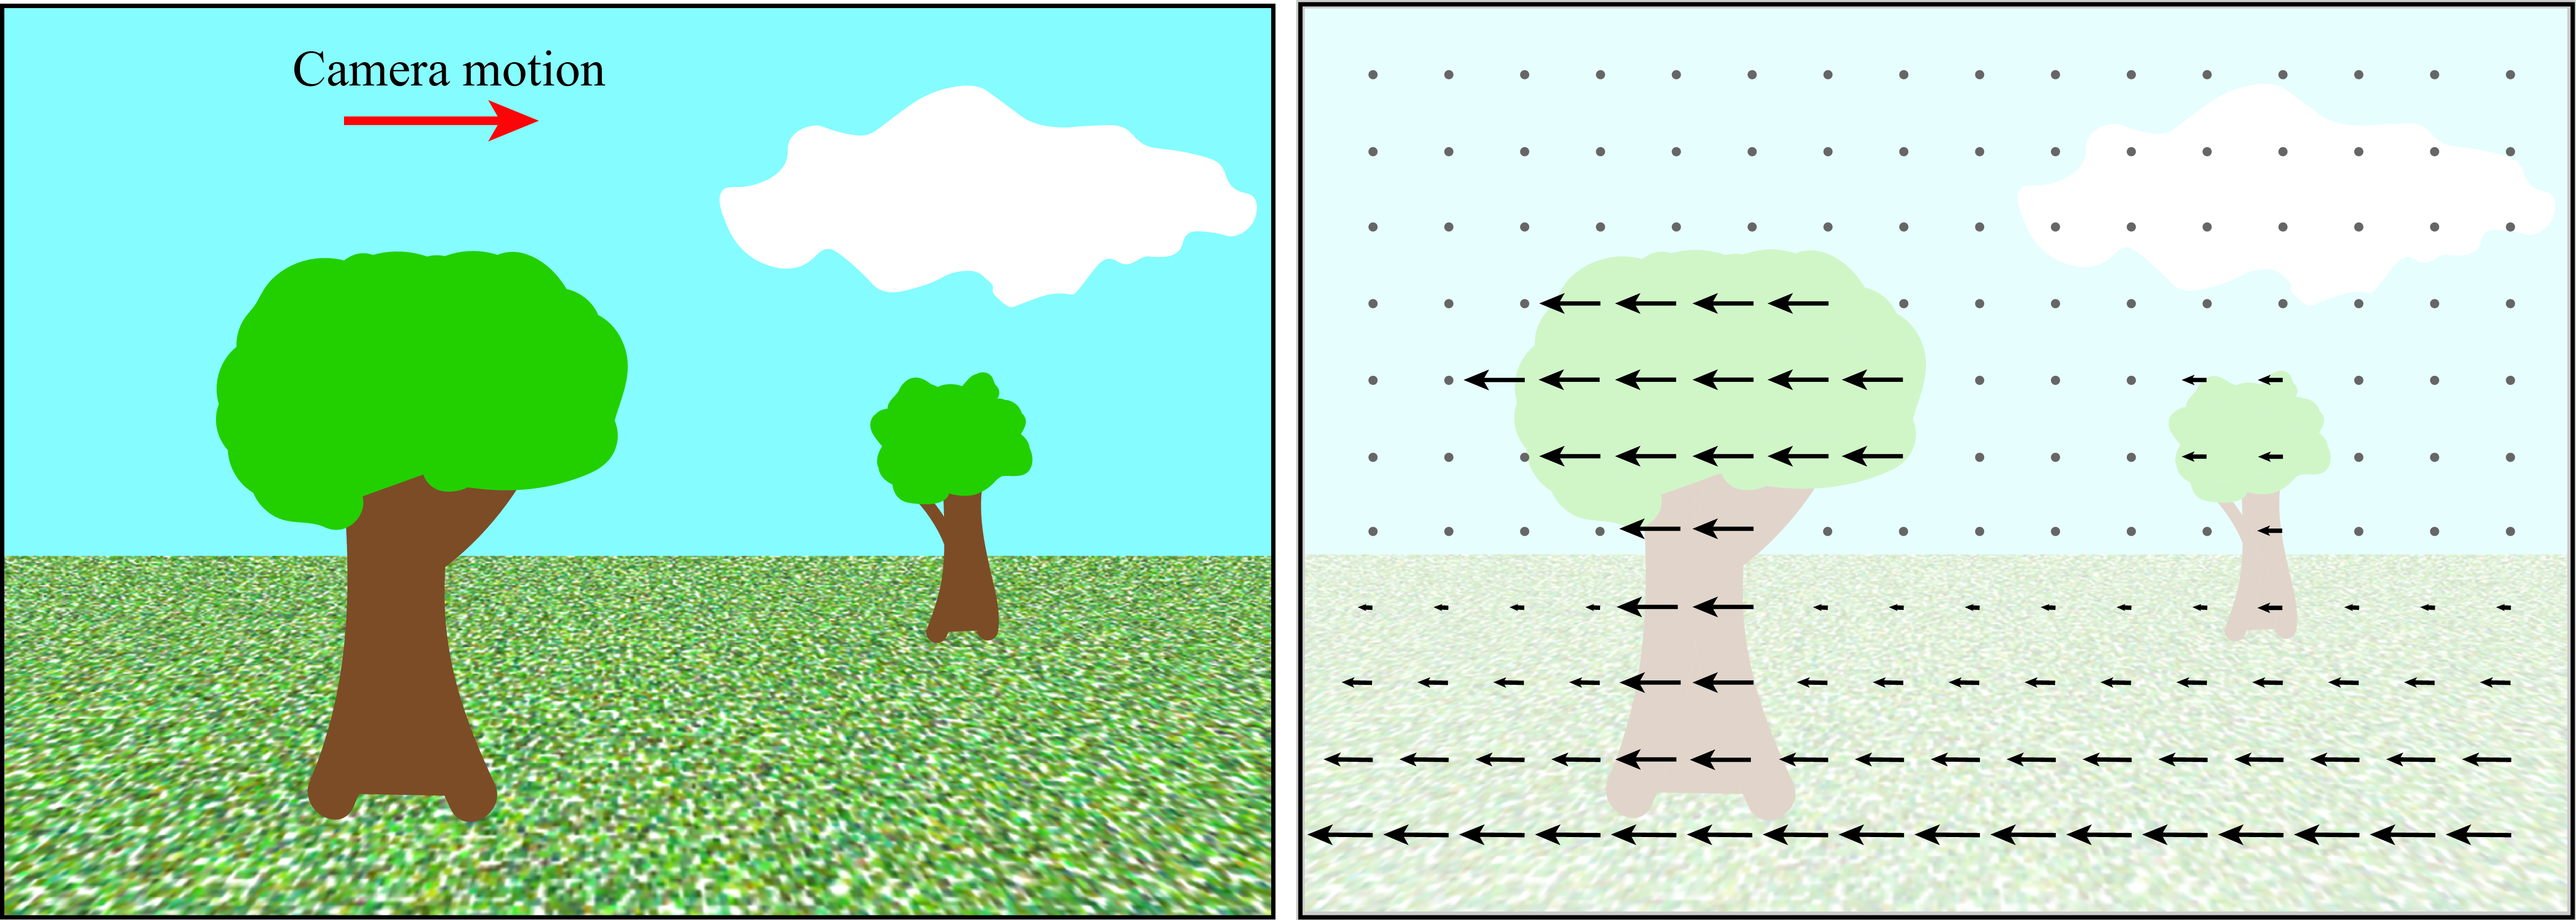
\includegraphics[width=1\linewidth]{figures/optical_flow/camera_lateral_translation_flow.eps}
    }
    \caption{Sketch of the motion field under lateral camera motion. Objects close to the camera will appear to be moving faster than objects farther away. Objects that are very far (like the cloud) will appear to be nearly stationary.}
    \label{fig:camera_lateral_translation_flow}
\end{figure}

\subsubsection{Camera forward motion and focus of expansion}
%~\\
For a camera moving forward, as illustrated in \fig{\ref{fig:camera_forward_translation}}, note that $V_X = V_Y = 0$. In this case, the motion is only along the $Z$-axis, $V_Z \neq 0$.

\begin{figure}[h!]
    \centerline{
        \includegraphics[width=1\linewidth]{figures/optical_flow/camera_forward_translation.eps}
    }
    \caption{Camera moving forward, along the camera axis.}
    \label{fig:camera_forward_translation}
\end{figure}

Using \eqn{\ref{eq:forward_objects}}, we get:
%\begin{eqnarray}
%\dot{x} & = &  \frac{V_Z}{Z}x \\
%\dot{y} & = &  \frac{V_Z}{Z}y
%\label{eq:motionprojection}
%\end{eqnarray}

\begin{align}
    \begin{bmatrix}
        \dot{x} \\
        \dot{y}
    \end{bmatrix}
    =
    \frac{V_Z}{Z}
    \begin{bmatrix}
        x \\
        y
    \end{bmatrix}
    \label{eq:motion_projection_focus_expansion}
\end{align}



\Eqn{\ref{eq:motion_projection_focus_expansion}} provides a few interesting insights. First, the rate of expansion does not depend on the focal length $f$. Second, the observed motion only depends on the ratio $V_Z/Z$, which is the inverse of the {\bf time to contact}.
\index{Time to contact}
The time to contact, $V_Z/Z$, is the time it will take the camera to reach the object located a distance $Z$ when moving at velocity $V_Z$.


For a camera moving in an arbitrary direction, that is, with $V_X \neq 0$, $V_Y \neq 0$, and $V_Z \neq 0$,  using \eqn{\ref{eq:motionprojection}} and \eqn{\ref{eq:motionvanishingpoint}} we get:

%\begin{eqnarray}
%\dot{x} & = &  \frac{-f V_X + V_Z x}{Z} = (x-x_{\infty}) \frac{V_Z}{Z}\\
%\dot{y} & = &  \frac{-f V_Y + V_Z y}{Z} = (y-y_{\infty}) \frac{V_Z}{Z}
%\label{eq:motionprojection_translation}
%\end{eqnarray}

\begin{align}
    \begin{bmatrix}
        \dot{x} \\
        \dot{y}
    \end{bmatrix}
    %= 
    %\frac{1}{Z}
    %\begin{bmatrix}
    %-f & 0 & x \\
    %0 & -f & y  
    %\end{bmatrix}
    %\begin{bmatrix}
    %V_X\\
    %V_Y \\
    %V_Z 
    %\end{bmatrix}
    =
    \frac{V_Z}{Z}
    \begin{bmatrix}
        x - x_{\infty} \\
        y - y_{\infty}
    \end{bmatrix}
    %\label{eq:motionprojection_translation}
\end{align}


The observed motion is zero at the {\bf focus of expansion}, $(x_{\infty}, y_{\infty})$. \index{Focus of expansion}

\Fig{\ref{fig:camera_forward_translation_flow}} illustrates the apparent motion field for a camera moving toward the center of a wall. Points near the center (which will be the point of impact) appear stationary, while points in the periphery appear to move faster and away from the center. The whole wall expands over time.

\begin{figure}[h!]
    \centerline{
        \includegraphics[width=1\linewidth]{figures/optical_flow/camera_forward_translation_flow.eps}
    }
    \caption{Sketch of the motion field when the camera approaches a planar surface. The motion field indicates the rate of expansion of the image, and it is a function of the time to contact. In this example, the focus of expansion is on the center.}
    \label{fig:camera_forward_translation_flow}
\end{figure}

\subsection{Camera Rotation}

Let's consider a general camera motion undergoing both translation and rotation. To compute the motion field with a compact expression, we will do a number of simplifications assuming a small motion between consecutive frames. After a small time interval, $\Delta t$, the camera will move, generating a displacement in the points with respect to the camera coordinate system equal to:

\begin{equation}
    \mathbf{P}_{t+\Delta t} = - \mathbf{T}_{\Delta t}  + \mathbf{R}_{\Delta t} \mathbf{P}_t
\end{equation}
where $\mathbf{T}_{\Delta t}$ is the camera translation and $\mathbf{R}_{\Delta t}$ is the camera rotation that took place over that time interval, $\Delta t$. The velocity of a 3D point with respect to the camera will be:
\begin{equation}
    \dot{\mathbf{P}} = \frac{\mathbf{P}_{t+\Delta t} - \mathbf{P}_{t}}{\Delta t} = - \mathbf{V} + \frac{\mathbf{R}_{\Delta t} -\mathbf{I}}{\Delta t} \mathbf{P}_t
    \label{eq:general_camera_motion_equation_full}
\end{equation}

To derive the rotation, we consider the {\bf Euler angles} \index{Euler angles} (\fig{\ref{fig:yaw_pitch_roll}}) and decompose the rotation using rotations along the three axes (yaw, pitch, roll):
\begin{figure}[h!]
    \centerline{
        \includegraphics[width=.4\linewidth]{figures/optical_flow/yaw_pitch_roll.eps}
    }
    \caption{Rotation expressed by Euler angles (yaw, pitch, roll).}
    \label{fig:yaw_pitch_roll}
\end{figure}

Each angle measures the rotation along the camera-coordinate axes. Using this representation of the rotation, the rotation matrix can be written as:
\begin{align}
    \mathbf{R}_{\Delta t} =
    \begin{bmatrix}
        \cos \theta_Z  & \sin \theta_Z & 0 \\
        -\sin \theta_Z & \cos \theta_Z & 0 \\
        0              & 0             & 1
    \end{bmatrix}
    \begin{bmatrix}
        \cos \theta_Y & 0 & -\sin \theta_Y \\
        0             & 1 & 0              \\
        \sin \theta_Y & 0 & \cos \theta_Y
    \end{bmatrix}
    \begin{bmatrix}
        1 & 0              & 0             \\
        0 & \cos \theta_X  & \sin \theta_X \\
        0 & -\sin \theta_X & \cos \theta_X
    \end{bmatrix}
\end{align}
In this equation, the sign of the angles are chosen to reflect that a rotation of the camera is equivalent to the opposite rotation of the 3D point.

For a small $\Delta t$, the angles will be small, and we can approximate the trigonometric functions, $\cos$ and $\sin$, by $\cos \alpha \approx 1$ and $\sin \alpha \approx \alpha$. We can also approximate the product $\sin \alpha \sin \beta \approx 0$ as it will result in a second-order term.

\begin{align}
    \mathbf{R}_{\Delta t} \approx
    \begin{bmatrix}
        1         & \theta_Z & 0 \\
        -\theta_Z & 1        & 0 \\
        0         & 0        & 1
    \end{bmatrix}
    \begin{bmatrix}
        1        & 0 & -\theta_Y \\
        0        & 1 & 0         \\
        \theta_Y & 0 & 1
    \end{bmatrix}
    \begin{bmatrix}
        1 & 0         & 0        \\
        0 & 1         & \theta_X \\
        0 & -\theta_X & 1
    \end{bmatrix}
    \approx
    \begin{bmatrix}
        1         & \theta_Z  & -\theta_Y \\
        -\theta_Z & 1         & \theta_X  \\
        \theta_Y  & -\theta_X & 1
    \end{bmatrix}
\end{align}

\begin{equation}
    \mathbf{P}_{t+\Delta t} - \mathbf{P}_{t} = - \mathbf{T}_{\Delta t} + (\mathbf{R}_{\Delta t} - \mathbf{I}) \mathbf{P}_t =
    - \mathbf{T}_{\Delta t} -
    \begin{bmatrix}
        0         & -\theta_Z & \theta_Y  \\
        \theta_Z  & 0         & -\theta_X \\
        -\theta_Y & \theta_X  & 0
    \end{bmatrix}
    \mathbf{P}_t
\end{equation}
The last term corresponds to the cross product in matrix form (note that we changed the sign of the matrix to make the cross product form more obvious). Therefore, we can rewrite the previous expression as:
\begin{equation}
    \mathbf{P}_{t+\Delta t} - \mathbf{P}_{t} =
    - \mathbf{T}_{\Delta t} - \bm{\theta} \times \mathbf{P}_t
\end{equation}
where $\bm{\theta}=(\theta_X,\theta_Y, \theta_Z)$. Substituting this expression into \eqn{\ref{eq:general_camera_motion_equation_full}}, we get the expression of the motion of a 3D point:
\begin{equation}
    \dot{\mathbf{P}} = - \mathbf{V} - \mathbf{W} \times \mathbf{P}_t =
    -\begin{bmatrix}
        V_X \\
        V_Y \\
        V_Z
    \end{bmatrix}
    -
    \begin{bmatrix}
        -W_Z Y + W_Y Z \\
        W_Z X - W_X Z  \\
        -W_Y X + W_X Y
    \end{bmatrix}
\end{equation}
where $\mathbf{W}$ is the angular velocity $\mathbf{W}=(W_X,W_Y,W_Z)$. Now we are ready to compute the 2D motion field by using \eqn{\ref{eq:motionprojection}}:
\begin{align}
    \begin{bmatrix}
        \dot{x} \\
        \dot{y}
    \end{bmatrix}
    = -\frac{1}{Z}
    \begin{bmatrix}
        f & 0 & -x \\
        0 & f & -y
    \end{bmatrix}
    \begin{bmatrix}
        V_X \\
        V_Y \\
        V_Z
    \end{bmatrix}
    -\frac{1}{Z}
    \begin{bmatrix}
        f & 0 & -x \\
        0 & f & -y
    \end{bmatrix}
    \begin{bmatrix}
        -W_Z Y + W_Y Z \\
        W_Z X - W_X Z  \\
        -W_Y X + W_X Y
    \end{bmatrix}
\end{align}

This expression can be rewritten as, using $x=f \, X/Z$ and $y=f \, Y/Z$:
\begin{align}
    \begin{bmatrix}
        \dot{x} \\
        \dot{y}
    \end{bmatrix}
    = \frac{1}{Z}
    \begin{bmatrix}
        -f & 0  & x \\
        0  & -f & y
    \end{bmatrix}
    \begin{bmatrix}
        V_X \\
        V_Y \\
        V_Z
    \end{bmatrix}
    +
    \frac{1}{f}
    \begin{bmatrix}
        xy      & -f^2-x^2) & f y  \\
        f^2+y^2 & -xy       & -f x
    \end{bmatrix}
    \begin{bmatrix}
        W_X \\
        W_Y \\
        W_Z
    \end{bmatrix}
    \label{eq:2d_motion_field_from_translation_and_rotation}
\end{align}
This is the expression we were looking for. It relates the 2D motion field with the camera velocity and rotation. The matrices are only a function of the intrinsic camera parameters (focal length, $f$) and the camera coordinates. Note that this expression is only valid for small displacements.

In the previous section we saw what happens when there is no rotation; now we can focus on the case when there is only camera rotation, that is $V_X=V_Y=V_Z=0$,
\begin{align}
    \begin{bmatrix}
        \dot{x} \\
        \dot{y}
    \end{bmatrix}
    =
    \frac{1}{f}
    \begin{bmatrix}
        xy      & -f^2-x^2) & f y  \\
        f^2+y^2 & -xy       & -f x
    \end{bmatrix}
    \begin{bmatrix}
        W_X \\
        W_Y \\
        W_Z
    \end{bmatrix}
\end{align}

The first thing to notice is that the 2D motion field does not depend on the 3D scene structure, $Z$, and it is only a function of the rotational velocity and the camera parameters. Therefore, under camera rotation we can not learn anything about the scene by observing the motion field. The only thing we can learn from the 2D motion field is about the motion of the camera.

Let's consider first rotation along the camera optical axis, that is $W_X=W_Y=0$. In this case the motion field is:
\begin{align}
    \begin{bmatrix}
        \dot{x} \\
        \dot{y}
    \end{bmatrix}
    =
    \begin{bmatrix}
        y \\
        -x
    \end{bmatrix}
    W_Z
\end{align}
The 2D motion field at each location $(x,y)$ will point in the orthogonal direction to the vector that connects that point with the origin (\fig{\ref{fig:motion_wz}}). The motion field does not depend on the focal length, $f$.

\begin{figure}[h!]
    \centerline{
        \includegraphics[width=.4\linewidth]{figures/optical_flow/motion_wz.eps}
    }
    \caption{Motion field for a rotating camera around the optical axis, $W_X=W_Y=0$.}
    \label{fig:motion_wz}
\end{figure}

If $W_Z=0$, then the rotation along $W_X$ or $W_Y$ will produce similar 2D motion fields, so let's consider $W_X=0$. We have:
\begin{align}
    \begin{bmatrix}
        \dot{x} \\
        \dot{y}
    \end{bmatrix}
    =
    -\frac{1}{f}
    \begin{bmatrix}
        f^2+x^2 \\
        xy
    \end{bmatrix}
    W_Y
\end{align}
In this case, the focal length $f$ will have a strong effect on the appearance of the motion field. For very large $f$, we can approximate the 2D motion field by $\dot{x} \approx f W_Y$ and $\dot{y} \approx 0$. The resulting motion field is approximately constant across the entire image and looks like lateral translation motion. For very small $f$, the motion field will be similar to the one produced by a homography and it will be very different to a lateral camera motion. The flows shown in \fig{\ref{fig:motion_wy_f03_f1_f3}} correspond to $f=1/3$, $f=1$, and $f=3$.


\begin{figure}[h!]
    \centerline{
        \includegraphics[width=1\linewidth]{figures/optical_flow/camera_motion_field_rotation_three_f.eps}
        %\includegraphics[width=.3\linewidth]{figures/optical_flow/motion_wy_f03.eps}
        %~\includegraphics[width=.3\linewidth]{figures/optical_flow/motion_wy_f1.eps}
        %~\includegraphics[width=.3\linewidth]{figures/optical_flow/motion_wy_f3.eps}
    }
    \caption{Motion flows corresponding to a rotation around the
        $Y$-axis. (left) $f = 1/3$. (middle) $f = 1$.
        (right) $f = 3$.}
    \label{fig:motion_wy_f03_f1_f3}
\end{figure}

Camera rotation around the $Y$-axis does not inform about the scene structure, but it informs about the camera parameters. The magnitude of $W_Y$ only affects the scaling of the motion vectors, but it does not change their orientation.

In the case of camera rotation, for a large angle (or a large $\Delta t$), the relationship between the image at time $t$ and the image at time $t+\Delta t$ is a homography.

%Rotation: camera rotation induces an optical flow that is independent of the 3D. 



%\subsection{Time to contact}

%It is an interesting example to understand the invariances of what is lost between 2D flow and 3D flow. 

\subsection{Motion under Varying Focal Length}

Before moving into motion estimation, let's consider one final scenario: a static camera observing a static scene, but the focal length changes over time. What will the motion field be?  In this setting, despite that there is not motion in the scene, the focal length of the camera changes over time, producing motion in the image plane. If the focal length increases, it will seem as if we are zooming into the scene. Would it be similar to a forward motion?

Starting from the perspective projection equation,
\begin{align}
    \begin{bmatrix}
        x \\
        y
    \end{bmatrix}
    = \frac{f}{Z}
    \begin{bmatrix}
        X \\
        Y
    \end{bmatrix}
    \label{eq:pers_proj}
\end{align}
If we compute the temporal derivative where only $f$ varies over time, we get:
\begin{align}
    \begin{bmatrix}
        \dot{x} \\
        \dot{y}
    \end{bmatrix}
    = \frac{\dot{f}}{Z}
    \begin{bmatrix}
        X \\
        Y
    \end{bmatrix}
    =
    \frac{\dot{f}}{f}
    \begin{bmatrix}
        x \\
        y
    \end{bmatrix}
\end{align}

The last expression is obtained by using \eqn{\ref{eq:pers_proj}}. As the equation shows, changing the focal length only results in a scaling of the projected image on the image plane. It does not create any parallax. As the sensor has finite size, changing the focal length results in a zoom and a crop. The motion field does not depend on the 3D scene structure. Therefore, images taken by a pinhole camera from the same viewpoint but with different focal lengths do not provide depth information about the scene. This is an example where there is a 2D motion field even when there is no motion in the scene.

\section{Concluding Remarks}

As we did in \chap{\ref{chapter:imaging}}, in this chapter we have focused on formulating the problem of image formation: How does the 3D motion in the world appear once it is projected on the image plane?

But the goal of vision is to inverse this projection and recover the 3D scene structure. In the upcoming chapters, we will proceed on the path begun in  \chap{\ref{chapter:motion_estimation}}, and we will study how to estimate motion from pixels.

%Now that we have studied how 3D object motion and camera motion project into the camera producing a 2D motion field, let's now focus on the problem of estimating the 2D motion field from image sequences. 
